%Kelompok BSD
%Arjun Yuda Firwanda
%Dwi Septiani Tsaniyah
%Dwi Yulianingsih
%Ervanda Rambu Anarky
%Jeremia Wahyudi Sianturi

\documentclass{article}

\usepackage{amsmath}
\usepackage{textcomp}
\usepackage{graphicx}
\usepackage{enumitem}
\usepackage{verbatim}

\begin{document}

Testing Kode Program Sensor Gerak

\section {Testing Program}
Sistem Testing (pengujian)

\begin{figure}[ht]
\centerline{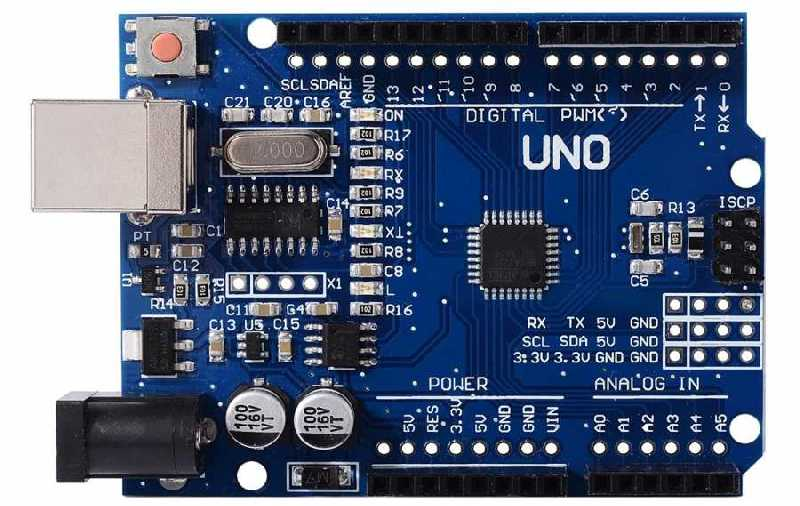
\includegraphics[width=1\textwidth]{figures/arduino.JPG}}
\caption{gambar arduino.}
\label{arduino.JPG}
\end{figure}
\ref{arduino}

Dalam \cite{evans2013arduino} Pengujian perangkat lunak (bahasa Inggris: software testing) merupakan suatu investigasi yang dilakukan untuk mendapatkan informasi mengenai kualitas dari produk atau layanan yang sedang diuji (under test).Pengujian perangkat lunak juga memberikan pandangan mengenai perangkat lunak secara obyektif dan independen, yang bermanfaat dalam operasional bisnis untuk memahami tingkat risiko pada implementasinya. Teknik-teknik pengujian mencakup, namun tidak terbatas pada, proses mengeksekusi suatu bagian program atau keseluruhan aplikasi dengan tujuan untuk menemukan bug perangkat lunak (kesalahan atau cacat lainnya).
Dalam dunia software perubahan requiretment adalah hal yang sangat biasa dan sulit ditebak maupun dihindari, dapat dipastikan karena adanya kesalahan-kesalahan pada software maupun pengguna dalam menganalisis objek yang ada. Sebuah metodelogi dalam pengembangan perangkat lunak yang dirancang untuk kondisi yang serba dinamis dan tidak terprediksi seperti masalah perubahan requiretment pada intinya akan kembali pada cara agar pengembangan sofware testing kode dapat berjalan dengan baik dan memberi feedback yang sesuai agar kesalahan yang ada dapat di minimalisir.
Secara sederhana, sketch yang ada dalam program Arduino dikelompokkan menjadi 3 blok 
\begin{enumerate}
\item Header	: Bagian header ini biasanya ditulis dengan definisi-definisi penting yang akan digunakan dalam program, misalnya pada penggunaan library dan pendefinisian variable. Code dalam blok ini dijalankan hanya sekali pada waktu.
\item Setup	: Di sinilah awal program Arduino berjalan, yaitu ketika power on Arduino board. Biasanya di blok ini diisi penentuan apakah suatu pin digunakan sebagai input atau output, menggunakan perintah pinMode. Initialisasi variable juga bisa dilakukan di blok ini
\item Loop	: bagian ini akan dicoba secara terus menerus. Apabila program sudah sampai pada tahap akhir blok, maka dilanjutkan dengan mengulang percobaan dari awal blok. Program akan berhenti apabila tombol Arduino di matikan. fungsi utama program Arduino berada.
\end{enumerate}

\subsection {Cara Merakit Sensor Pir}

Alat yang diperlukan:
\begin{enumerate}
\item Arduino Uno.
\item Sensor Pir.
\item Lampu Led (warna bebas).
\item Kabel Jumper Male to Female (3 buah warna).
\item Kabel USB.
\item PC.
\end{enumerate}

Cara Merakit:
Gabungkan kabel jumper male to female berwarna orange dari VCC sensor pir ke pin 5 arduino.

\ref{kabelvcc}

\begin{figure} {ht}
\centerline{\includegraphics{width=1\textwidth}{figures/kabelvcc.JPG}}
\caption{gambar kabelvcc.}
\label{kabelvcc.JPG}
\end{figure}


Gabungkan kabel jumper male to female berwarna merah dari OUPUT sensor pir ke pin 3 arduino.

\ref{kabeloutput}
\begin{figure} {ht}
\centerline{\includegraphics{width=1\textwidth}{figures/kabeloutput.JPG}}
\caption{gambar kabeloutput.}
\label{kabeloutput.JPG}
\end{figure}


Gabungkan kabel jumper male to female berwarna coklate dari GND sensor pir ke GND arduino.

\ref{kabelgnd}
\begin{figure} {ht}
\centerline{\includegraphics{width=1\textwidth}{figures/kabelgnd.JPG}}
\caption{gambar kabelgnd.}
\label{kabelgnd.JPG}
\end{figure}


Pasang lampu led berwarna biru ke pin 13 arduino.

\ref{led}
\begin{figure} {ht}
\centerline{\includegraphics{width=1\textwidth}{figures/led.JPG}}
\caption{gambar led.}
\label{led.JPG}
\end{figure}


Pasang kabel USB dari arduino ke PC.

\ref{kabelusb}
\begin{figure} {ht}
\centerline{\includegraphics{width=1\textwidth}{figures/kabelusb.JPG}}
\caption{gambar kabelusb.}
\label{kabelusb.JPG}
\end{figure}


Process software testing merupakan process yang sangat penting dalam dunia perangkat lunak. karena dengan kita menerapkan process ini di dalam alur pengembangan software kita, maka dengan ini kita dapat menjamin kualitas dari software yang kita buat (setidaknya dalam hal pemenuhan functional requirement). Lalu, apa saja process software testing yang harus kita lakukan? software developer dan baca-baca buku tentang software development, setidaknya ada 3 jenis testing yang dapat kita lakukan yaitu: Unit Testing, Integration Testing dan User Acceptance Testing (UAT)

Unit Testing
Unit testing adalah sebuah percobaan dalam sebuah project. Seorang programmer harus melakukan banyak testing sehingga apa-apa saja yang kurang tersebut harus mengetahuinya dan dapat mengevaluasi kebenaran datanya. Testing harus dilakukan secara bertahap dan dilakukan sebanyak mungkin untuk sebuah project. Programmer yang cerdas seharusnya dapat melakukan testing menurut teori dan diterapkan dalam sebuah praktik.
 
Integration Testing
Lain dengan unit testing yang memiliki sifat independen dan isolasi, Integration testing dibuat untuk uji coba apakah kerjasama dari satu fungsi dengan fungsi lainnya (baik dalam satu kelas maupun berbeda kelas) dapat menghasilkan output yang benar atau tidak. Dalam pelaksanaannya, proses integration testing tidak hanya dilakukan pada kode program yang dihasilkan oleh satu orang , akan tetapi melibatkan  kode-kode program yang dibuat oleh programmer lain juga.

User Acceptence Test (UAT)
Dalam melakukan User Acceptance Test (UAT) atau Uji Penerimaan Pengguna, client atau pemilik produk akan memeriksa apakah user interface, alur aplikasi dan data-data yang ditampilkan oleh aplikasi telah sesuai dengan requirement yang diinginkan ataukah tidak. Error yang ditemui pada tahap ini biasanya sulit diidentifikasi sumbernya serta output yang dihasilkan oleh fungsi dan class selalu berkomunikasi satu dan lainnya.
Satu hal yang harus diingat dalam melakukan unit testing tersebut adalah jika unit testing tersebut adalah testing yang bersifat independen dan isolated. Sebuah method / fungsi dapat dikatakan sebagai independen jika fungsi tersebut tidak bergantung dengan hasil dari fungsi yang lain sedangkan yang dimaksud dengan isolated adalah bahwa fungsi yang di test tidak boleh melakukan akses ke “luar” seperti misalnya mengakses database, file ataupun membutuhkan koneksi jaringan.


Menurut \cite{gifson2009sistem} Cara mengakses sensor PIR menggunakan Arduino yaitu

\ref{sensorpir}

\begin{figure}[ht]
\centerline{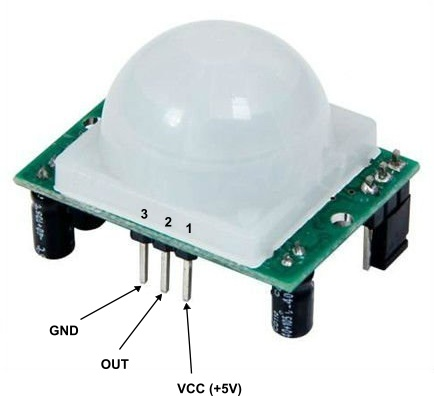
\includegraphics[width=1\textwidth]{figures/sensorpir.JPG}}
\caption{gambar sensorpir.}
\label{sensorpir.JPG}
\end{figure}

Sensor PIR (Passive Infra Red) atau disebut dengan Sensor Gerak merupakan sensor yang digunakan untuk mendeteksi adanya benda atau sebuah gerakan tangan untuk mentransfer dengan cara infra red atau sinar merah yang berasal dari gerakan tangan. Tidak hanya dengan pendeteksian pancaran sinar infra merah melaikan sebuah infra red.
Komponen elektronika ini mempunyai sifat pasif, yang artinya tidak dapat memancarkan sinar infra merah secara independen tetapi hanya menerima radiasi sinar infra merah dari luar.

Kegunaan dari sensor ini biasanya digunakan dalam perancangan detektor pergerakan. Dikarenakan semua benda yang memancarkan energi radiasi, akan terdeteksi oleh sensor ini pada saat infra merah dari sensor PIR mendeteksi dengan perbedaan suhu tertentu.

Contoh dalam kehidupan sehari – hari yaitu pada saat memasuki pintu Mall yang membuka dengan otomatis saat kita akan memasuki area dalam Mall.

Cara kerja pembacaan pada sensor PIR

\ref{pembacaansensorpir}

\begin{figure}[ht]
\centerline{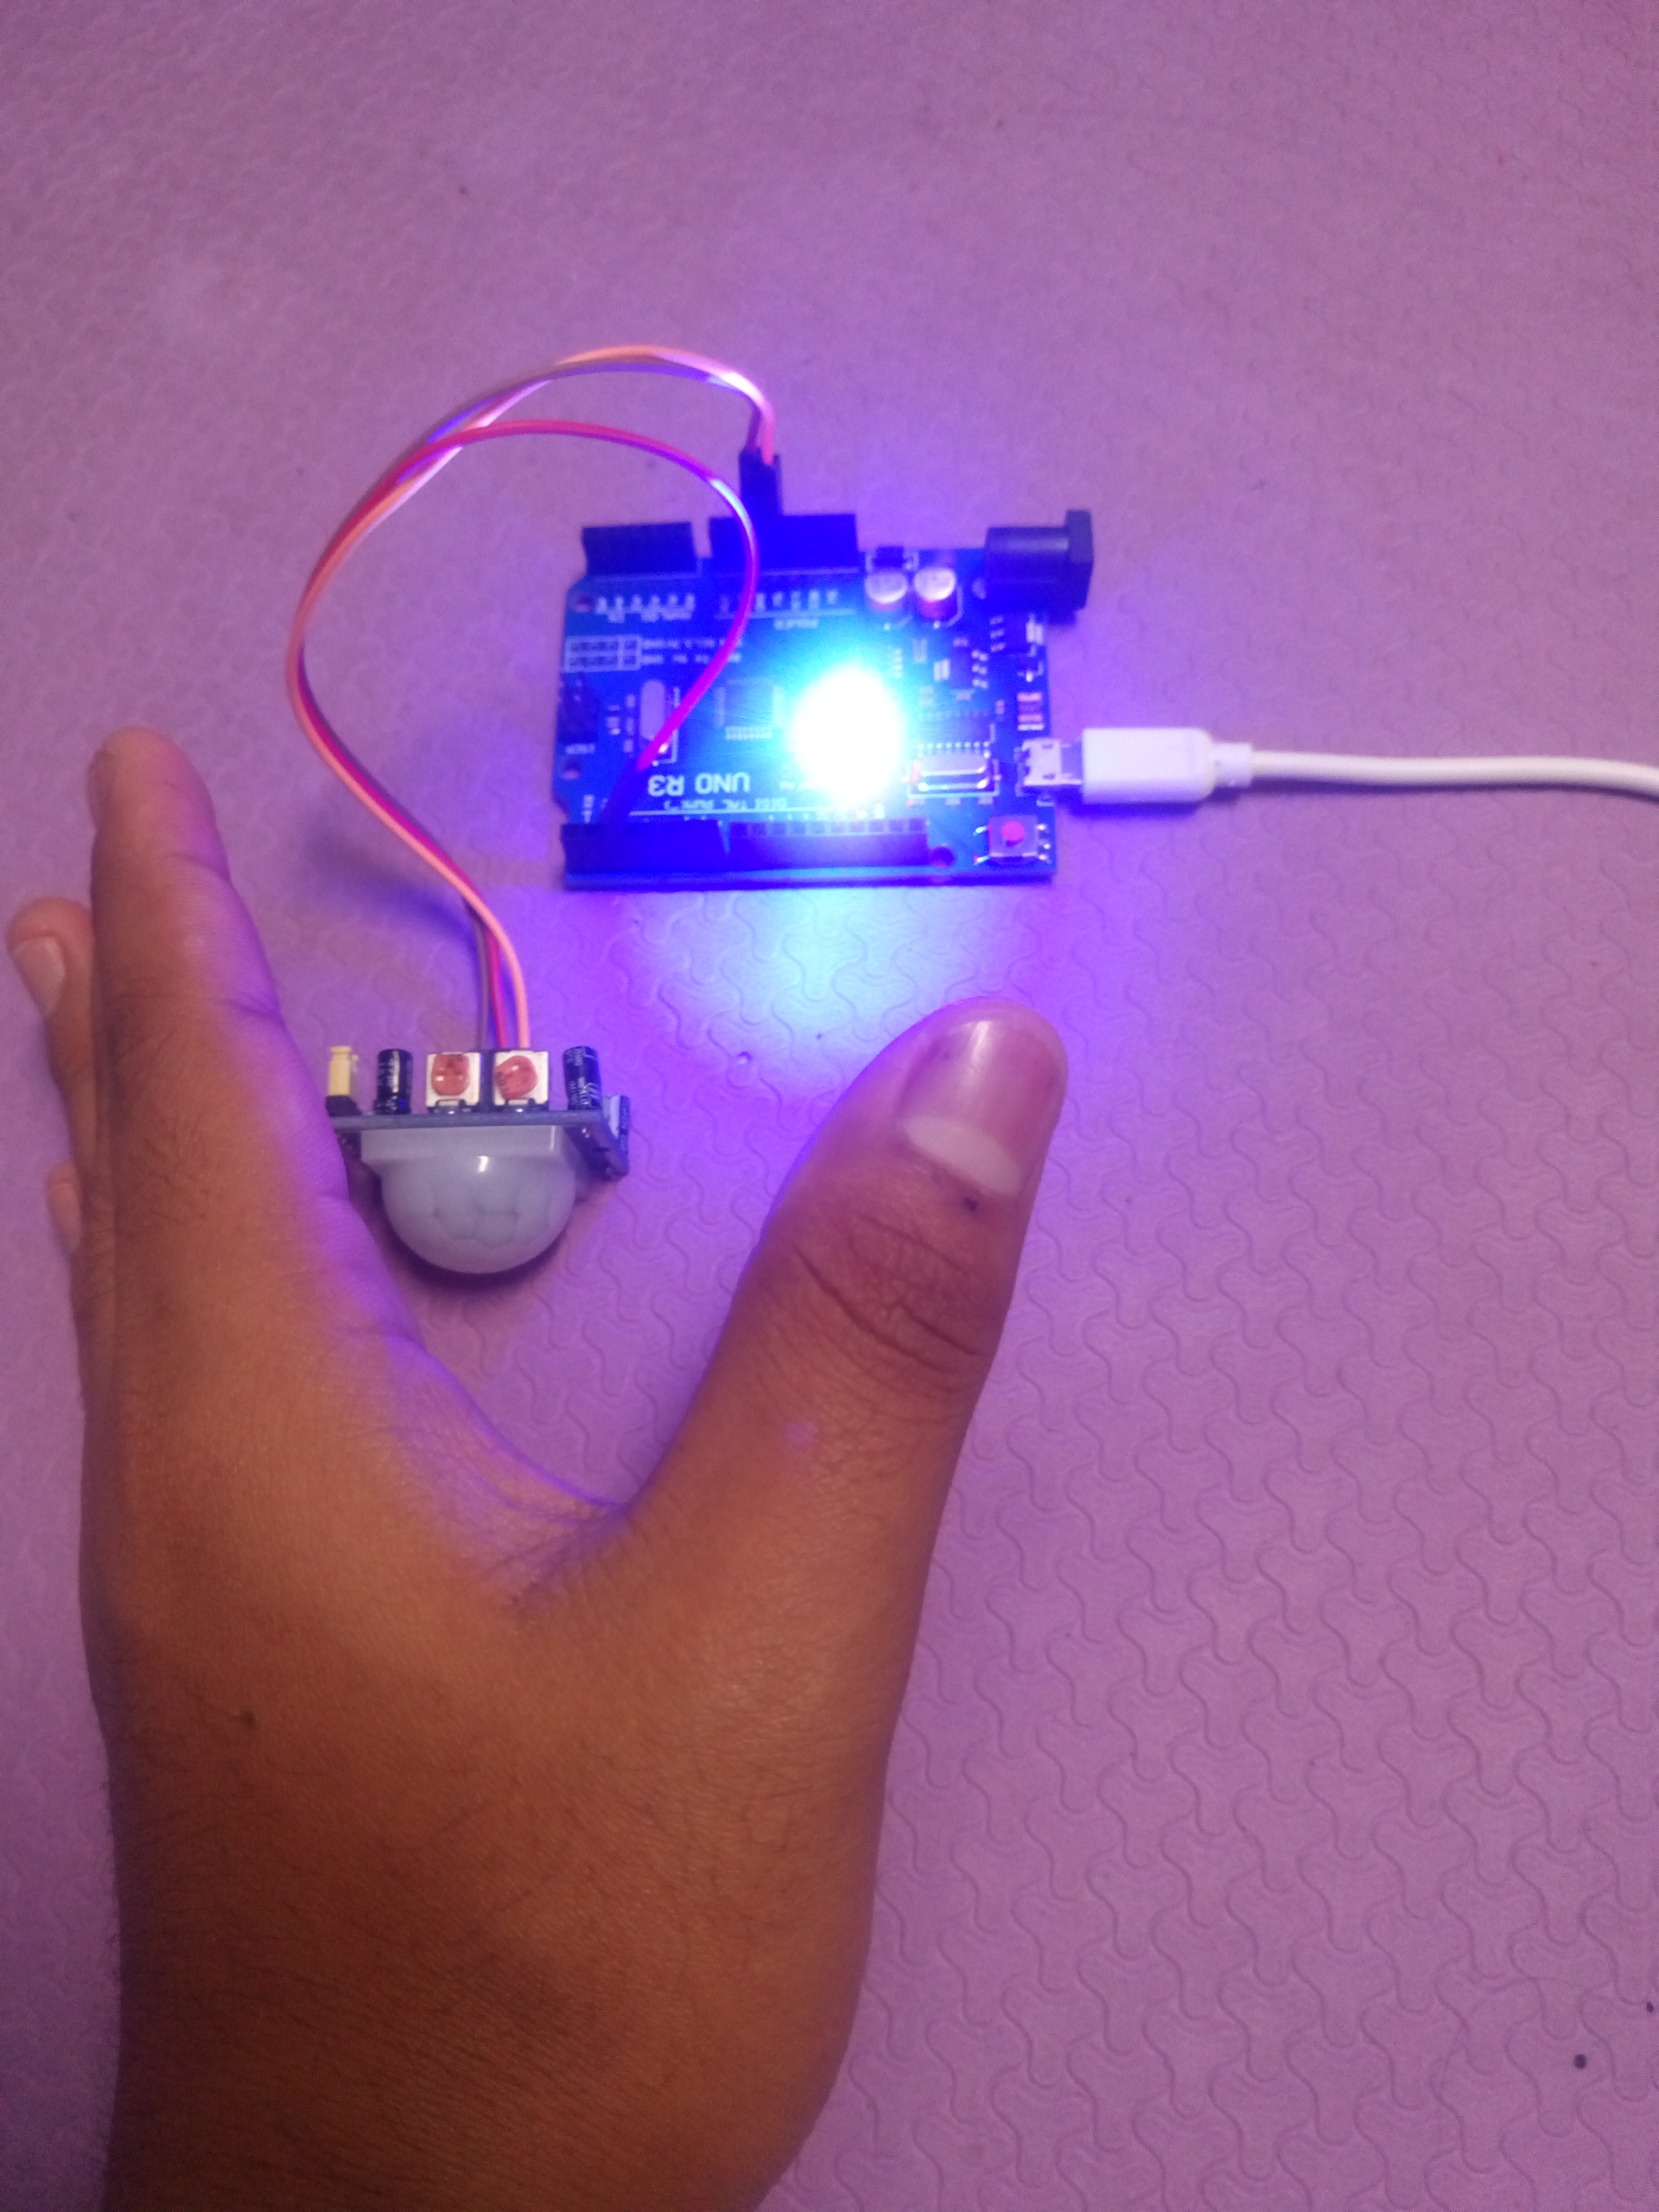
\includegraphics[width=1\textwidth]{figures/pembacaansensorpir.JPG}}
\caption{gambar pembacaansensorpir.}
\label{pembacaansensorpir.JPG}
\end{figure}

Pantulan dari infra merah yang telah masuk melalui lensa fresnel dan mengenai sensor akan menimbulkan energi panas dari energi panas tersebut maka sensor akan mengeluarkan arus listrik.
Sensor pyroelektrik tersebut disasari oleh beberapa bahan yang didalamnya mengandung galium nitrida (GaN), cesium nitrat (CsNo3) serta litium tantalate (LiTaO3).
Arus listriktersebut yang akan memunculkan tegangan analog yang kemudian dikenali oleh sensor. setelah itu sinyal akan dikuatkan dan dibandingkan oleh komparator dengan tegangan masing-masing (hasil yang diberikan berupa sinyal 1-bit).

Jadi sensor PIR hanya akan mengeluarkan logika 0 dan 1 saja. Jika logika 0, kondisi saat sensor tidak mendeteksi adanya pancaran infra merah dan sedangkan pada saat kondisi logika 1 kondisi saat sensor mendeteksi infra merah.

\ref{pintumall}

\begin{figure}[ht]
\centerline{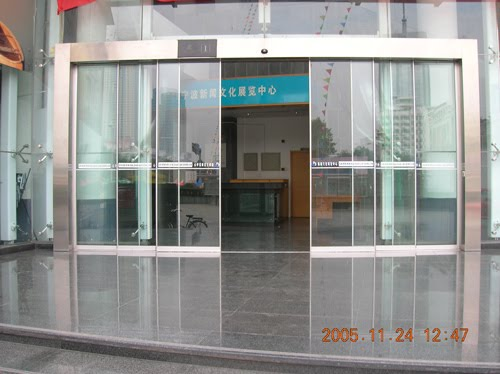
\includegraphics[width=1\textwidth]{figures/pintumall.JPG}}
\caption{gambar pintumall.}
\label{pintumall.JPG}
\end{figure}

Sensor PIR atau disebut dengan sensor gerak didesain dan dirancang sedemikian rupa untuk mendeteksi pancaran sinar infra merah dengan panjang gelombang 8 sampai14 mikrometer, diluar ukuran tersebut gelombang infra red sensor tidak akan mendeteksinya atau tidak dapat terbaca oleh sensor tersebut. Pendeteksian sensor PIR  dapat dilakukan dengan gerakan tangan, dengan cara menggerakkan tangan ke arah sensor PIR.
Pada kalangan manusia yang memiliki suhu badan, suhu tersebut adalah penyebab dimana manusia bisa menghasilkan sinar infra merah dengan panjang gelombang berkisar 9-10 mikrometer (nilai standar yang digunakan 9,4 mikrometer), dengan panjang gelombang tersebut maka akan terbaca oleh sensor PIR. Pada umumnya sensor tersebut memang dirancang agar dapat mendeteksi gerakan manusia yang kemudian bisa membuat sensor tersebut menyala atau berfungsi.

Pada saat sensor itu mulai terpasang dan sensor tidak bisa mendeteksi karena adanya benda yang bergerak di depannya maka lampu LED tersebut secara default akan langsung padam, dan sensor akan menyala lagi dalam waktu yang sangat delay yang telah diatur sedemikian rupa pada potensiometer sensor PIR (Passive Infra Red) .

\ref{kodeprogram}

\begin{figure}[ht]
\centerline{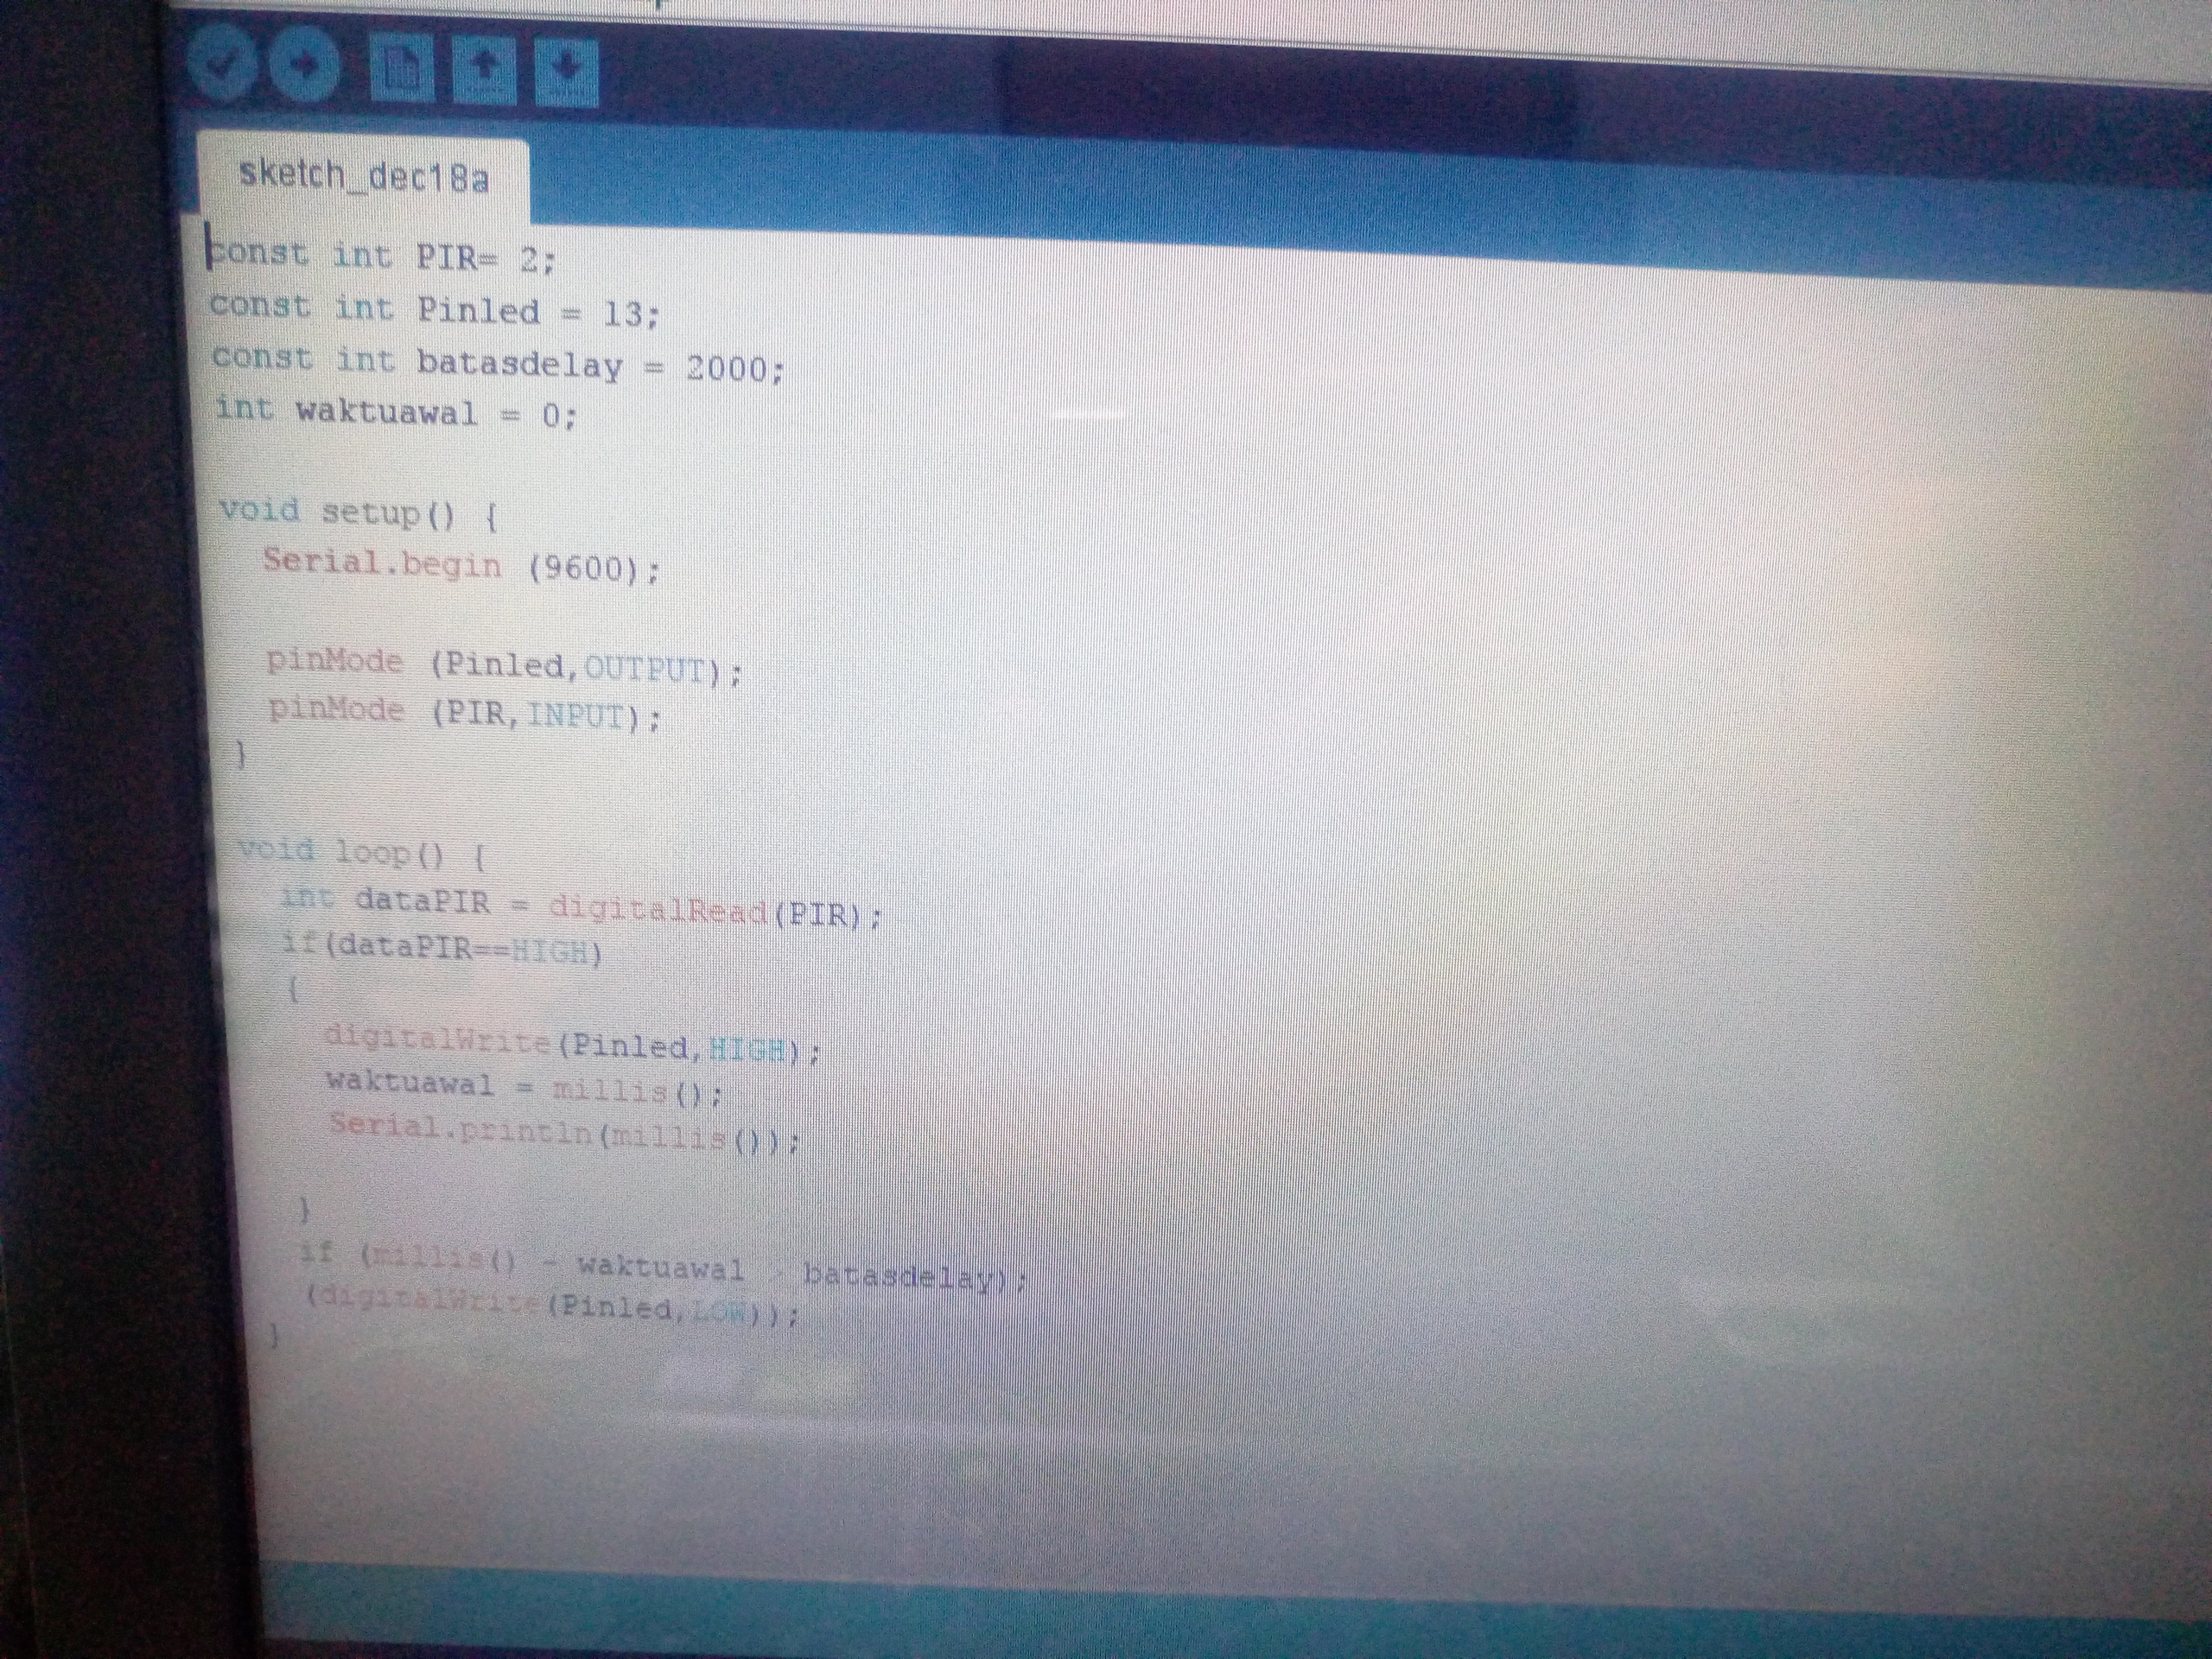
\includegraphics[width=1\textwidth]{figures/kodeprogram.JPG}}
\caption{gambar kodeprogram.}
\label{kodeprogram.JPG}
\end{figure}

Seperti itulah sedikin gambaran mengenai cara kerja sensor PIR atau sensor gerak yang akan berfungsi jika mendapatkan gerakan. dan gerakan itu akan direspon dalam infra merah sehingga PIR bisa langsung mendeteksi gerak tersebut. Dan jarak PIR dengan pusat gerak pun memiliki batas tersendiri dan tidak bisa terlampau jauh dari pusat gerakan karena PIR tidak akan merespon jika diluar jangkauan batas pusat gerakan.

\subsection {Cara kerja sensor suara}

Pada dasarnya sensor suara ialah sensor yang mendeteksi besarnya suara untuk diubah menjadi energi listrik. sensor ini akan bekerja berdasarkan pada besar maupun kecilnya suara yang akan diubah dan gelombang yang diterima dimana gelombang itu mengenai membran sensor dan terdeteksi oleh sensor yang membuat sensor bergerak. kumparan kecil yang dimiliki oleh sensor yang akan menghasilkan listrik yang kecepatannya bergantung pada gerak kumparan, gerak tersebut mempengaruhi besar kecilnya tenaga listrik yang di hasilkan contoh dari sensor ini adalah microphone.

\subsection {Prinsip Kerja Condeser}
Berdasarkan dengan susunan backplate condenser mic yang bekerja dengan diafragmayang harus dibantu oleh listrik membentuk sound sensitive kapasitor  Dengan gelombang suara yang masuk ke microphone akan mucul getar komponen diafragma ini. Letak dari diafragma ini sendiri di simpan tepat pada backplate. Susunan yang terdiri dari elemen ini membentuk sebuah kapasitor yang biasa disebut juga kondenser. Kapasitor ini memiliki kemampuan lebih untuk menyimpan suatu muatan maupun tegangan. Diantara diafragma dan ketika elemen tersebut diisi oleh muatan akan terbentuk suatu medan magnet dan backplate besarnya itu akan sangat professional terhadap ruang yang terbentuknya. Diafragma dengan backplate memiliki variasi yang akan lebar space yang disebabkan oleh adanya pergerakan diafragma yang relatif terhadap backplate yang disebabkan oleh adanya takanan suara yang mengenai diafragma. Oleh karena itu hal ini akan menghasilkan sinyal elektrik yang akan masuk pada condenser microphone

\ref{condenser.JPG}

\begin{figure}[ht]
\centerline{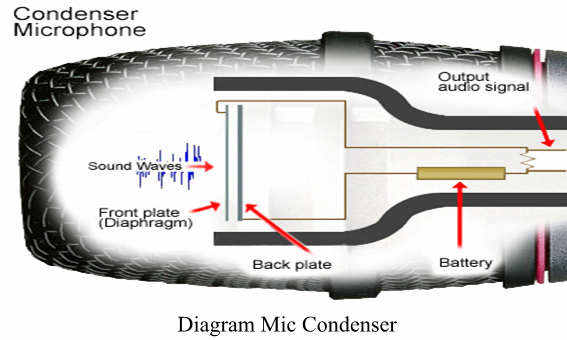
\includegraphics[width=1\textwidth]{figures/condenser.JPG}}
\caption{gambar condenser.}
\label{condenser.JPG}
\end{figure}

Karakteristik dari Condeser
\begin{enumerate}
\item Susunan kondeser lebih kompleks dibanding dengan jenis microphone lainnya dibanding dengan dynamic Microphone
\item Pada frekuensi tinggi, akan menghzxasilkan suara yang lebih halus dan natural, serta sensitivitas yang lebih tinggi
\item Mudah akan mencapai respon frekuensi flat dan memiliki range frekuensi yang lebih luas
\item Ukurannya lebih kecil dibanding dengan jenis tipe mikrophone lainnya
Pada pasaran sudah dijual sensor suara menggunakan condeser mic ini dalam bentuk modul, sehingga mudah dan praktis dalam penggunaannya.
\end{enumerate}

\subsection {Keuntungan dalam Melakukan Testing}
Ada tiga keuntungan yang didapat saat melakukan unit testing pada setiap kode yang dituliskan saat melakukan pengembangan suatu program.
\begin{enumerate}
\item Meminimalisir kesalahan pada saat program sudah berjalan (mode produksi), Karena kesalahan yang mungkin terjadi sudah diketahui saat masa dalam tahap pengembangan.
\item Perspektif unit testing, saat membuat kode yang testable secara tdak langsung membuat anda meningkatkan kemampuan dalam menulis kode dengan kualitas tinggi. Dengan begitu project akan terlihat hasilnya sesuai rencana.
\item Menjaga program yang anda tulis dari kerusakan di masa depan. Saat program anda semakin berkembang dengan fitur-fitur yang semakin banyak, maka unittesting akan memberi tahu anda jika ada nilai yang tidak sesuai dengan spesifikasi. Artinya pengembang dituntut untuk teliti dan memahami apa yang sedang dia kerjakan dalam projectnya.
\end{enumerate}

\subsection {Kekurangan dalam Melakukan Testing}
Ada beberapa kekurangan yang didapat dari melakukan testing kode program yang dituliskan saat melakukan pengembangan.
\begin{enumerate}
\item Kurangnya teliti atau kejelian dalam melakukan sebuah testing kode pada pengembangan sensor.
\item Kurangnya berhati-hati dalam melakukan percobaan, baik saat pengkodean dan pada sensor yang dikembangnya.
\item Kurangnya dalam memahami dari segi teori.
\item Kurangnya kerjasama dalam membuat pengembangan pada sebuah sensor.
\item Kurangnya komunikasi antara pengembang dan hasil yang didapat
\item Kurangnya kedisplinan dalam uji coba dan waktu yang diperlukan.
\item Kurangnya sempurnanya hasil yang didapat karena sebuah problem dalam pengembangannya.
\item Kurangnya melakukan pembahasan dengan dosen ataupun senior yang ada.
\item Kurangnya memanfaatkan waktu luang dalam pengerjaan sensor.
\item Kurangnya pengawasan saat melakukan pengembangan
\end{enumerate}

Dari beberapa kekurangan di atas dapat disimpulkan bahwa para pengembang harus melakukan sebuah rencana yang terperinci yang sebelumnya sudah berdasarkan teori dan pembahasan dengan dosen ataupun senior yang ada. Sebuah keharusan untuk para pengembang dalam pengujian baik dari segi sensor maupun kode yang digunakan untuk mengembangkan sebuah rencana.
Rencana yang baik dan terperinci akan menentukan sebuah hasil pengembangan sesuai yang dengan diharapkan semua pengembang.

\subsection { Perbedaan antara White Box Testing dengan Black Box Testing}
\begin{enumerate}
\item White Box Testing :
 Pengujian pada white box testing ini didasari oleh detail prosedur dan alur logika pada kode program. Pada kegiatan white box testing ini source program dilihat oleh tester dan menemukan kode program dari bugs. Intinya pada pengujian ini dilakukan sampai dengan pengecekan kode program. 
\item Black Box Testing : 
Pengujian pada black box testing yang didasari oleh detail aplikasi seperti tampilan aplikasi, fungsi yang ada didalam aplikasi dan sesuai dengan alur fungsi  dan dengan alur proses bisnis yang diinginkan oleh seorang costumer. Pengujian ini  tidak melihat dan menguji source pada kode programnya. 
\end{enumerate}
\end{document}